%!TEX root = ../thesis.tex
%*******************************************************************************
%*********************************** First Chapter *****************************
%*******************************************************************************

\chapter*{Introduction}  %Title of the First Chapter
\addcontentsline{toc}{chapter}{Introduction}

\ifpdf
    \graphicspath{{Introduction/Figs/}{Introduction/}}
\else
    \graphicspath{{Introduction/Figs/}{Introduction/}}
\fi

The natural process of evolution of mankind brought many changes. These changes are political, social, economic and especially environmental. The society development has brought with it changes in the environment and these changes were presented mainly by technological progress that spurred the improvement of the use of the environment and consequently brought its degradation. This is the reason why emerges studies focusing on the impacts of global environmental change as well as observations of the distribution of impacts of natural hazards and problems of land-use and land-cover change. 

Not neglecting the main driver of climate change as pollution, in the context of global change and sustainable development, deforestation still remains the second leading cause of greenhouse gas emissions \citep{culas11}. The world’s forests have a substantial role in the global carbon cycle. %\citet{FAO3} address the latest estimates for the terrestrial sink for the decade 1993-2003 at 3,300 MtCO2/yr, ignoring emissions from land-use change which represents a significant value of at least 33\% of the industrial sector emissions in 2004 (9,900 MtCO2).
Deforestation occurred in the temperate and sub-tropical areas in 19th and 20th centuries and are no longer significant in the developed temperate countries. Nowadays, it can be seen that temperate countries are now recovering their forest area which represents countries with upper middle and high incomes.

\begin{figure}[H]
\centering
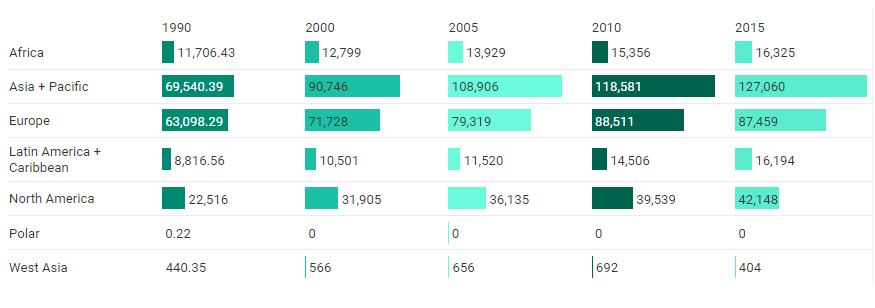
\includegraphics[width=1\linewidth]{Introduction/forestplantation.png}
\caption[Planted Forest Area from 1990 to 2015 in thousand of hectares]{Planted Forest Area from 1990 to 2015 in thousand of hectares. Forest plantation is a forest established by planting and/or seeding in the process of afforestation or reforestation. It consists of introduced species or, in some cases, indigenous species. Forest plantation and natural forests are included in the term forest, a term that refers to land with a tree cover of more than 10 percent and area of more than 0.5 ha. Forests are determined both by the presence of trees and the absence of other predominant land uses. The trees should be able to reach a minimum height of 5 m. Young stands that have not yet reached, but are expected to reach, a crown density of 10m percent and tree height of 5 m are included under forest, as are temporarily unstocked areas. The term includes forests used for purposes of production, protection, multiple use or conservation (i.e. forest in national parks, nature reserves and other protected areas), as well as forest stands on agricultural lands (e.g. windbreaks and shelterbelts of trees with a width of more than 20 m) and rubberwood plantations and cork oak stands. The term specifically excludes stands of trees established primarily for agricultural production, for example fruit tree plantations. It also excludes trees planted in agroforestry systems. Source: \citep{unep_2018}.}
\label{intro-fig:1}
\end{figure}

Tropical deforestation is a relatively modern event that gained momentum in the second half of the 20th century, more precisely, considerable deforestation in the world during 1990-2015 was almost entirely confined to the tropical regions. Figure \ref{intro-fig:2} shows the percentage of forested land in each region. Asia and Latin America had the highest net loss of forest during the period of 1990 to 2015. 

\begin{figure}[H]
\centering
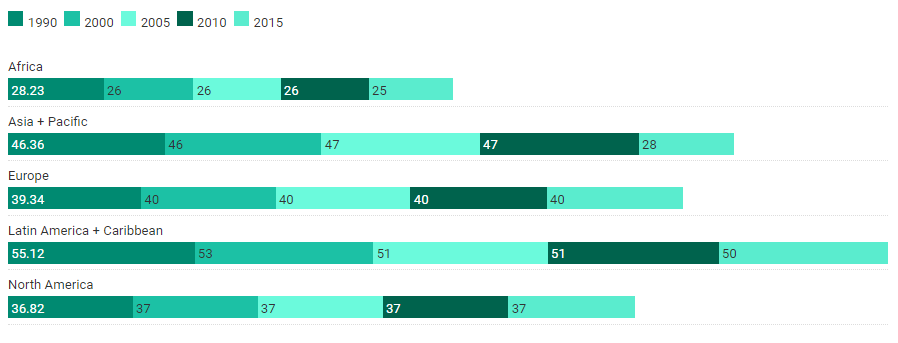
\includegraphics[width=1\linewidth]{Introduction/landcoveredbyforest.png}
\caption[Proportion of land covered by forest from 1990 to 2015 in percentage]{Proportion of land covered by forest from 1990 to 2015 in percentage. Forest: Land spanning more than 0.5 hectares with trees higher than 5 meters and a canopy cover of more than 10 percent, or trees able to reach these thresholds in situ. It does not include land that is predominantly under agricultural or urban land use. Explanatory notes 1. Forest is determined both by the presence of trees and the absence of other predominant land uses. The trees should be able to reach a minimum height of 5 meters in situ. Areas under reforestation that have not yet reached but are expected to reach a canopy cover of 10 percent and a tree height of 5 m are included, as are temporarily unstocked areas, resulting from human intervention or natural causes, which are expected to regenerate. 2. Includes areas with bamboo and palms provided that height and canopy cover criteria are met. 3. Includes forest roads, firebreaks and other small open areas; forest in national parks, nature reserves and other protected areas such as those of specific scientific, historical, cultural or spiritual interest. 4. Includes windbreaks, shelterbelts and corridors of trees with an area of more than 0.5 ha and width of more than 20 m. 5. Includes plantations primarily used for forestry or protection purposes, such as rubberwood plantations and cork oak stands. 6. Excludes tree stands in agricultural production systems, for example in fruit plantations and agroforestry systems. The term also excludes trees in urban parks and gardens. The term is mainly related to FRA 2005 National Reporting Table T1. Source: \citep{unep_2018}.}
\label{intro-fig:2}
\end{figure}

Figure 3 shows that total deforestation across Latin America remains concentrated
in Meso America and South America. This is not surprising, given that this area contains 86\% of the total tropical forest area found in Latin America. Actually, Brazil accounts for 60\% of Latin America’s tropical forests. Thus, the slowdown in deforestation in Brazil is largely responsible for the decline in overall tropical deforestation in Latin America. It is also possible to aggregate information from Figure 1, 2 and 3 in this process, lower middle income and upper middle income accounts for these developing countries from 1990-2000. The decrease in
planted forests means the increase in clearing areas, which corroborates for the scenario.
In other words, many low- and middle-income economies are rapidly changing land use, by converting forests, woodlands and other natural habitat to agriculture and other land-based development activities \citep{BARBIER2}.

\begin{figure}[H]
\centering
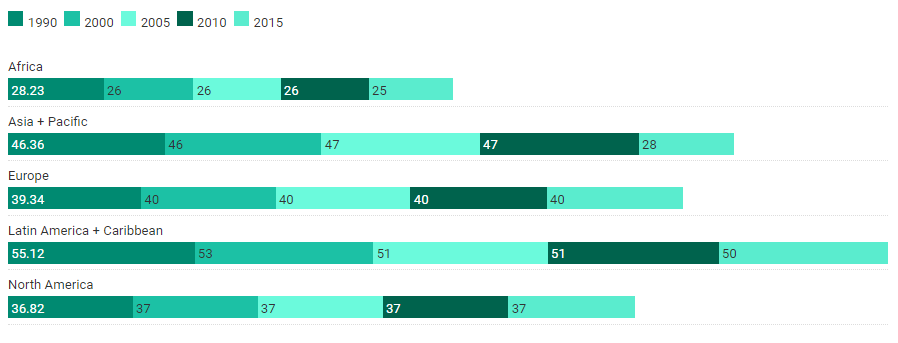
\includegraphics[width=1\linewidth]{Introduction/landcoveredbyforest.png}
\caption[Forest Average Annual Change from 1990 to 2015 in Thousand Hectares per Year.]{Forest Average Annual Change from 1990 to 2015 in Thousand Hectares per Year. Forest Average Annual Change – Total is the net change in forests and includes expansion of forest plantations and losses and gains in the area of natural forests. Total Forest includes natural forests and forest plantations. The term is used to refer to land with a tree cover of more than 10 percent and area of more than 0.5 ha. Forests are determined both by the presence of trees and the absence of other predominant land uses. The trees should be able to reach a minimum height of 5 m. Young stands that have not yet reached, but are expected to reach, a crown density of 10m percent and tree height of 5 m are included under forest, as are temporarily unstocked areas. The term includes forests used for purposes of production, protection, multiple use or conservation (i.e. forest in national parks, nature reserves and other protected areas), as well as forest stands on agricultural lands (e.g. windbreaks and shelterbelts of trees with a width of more than 20 m) and rubberwood plantations and cork oak stands. The term specifically excludes stands of trees established primarily for agricultural production, for example fruit tree plantations. It also excludes trees planted in agroforestry systems. Source: \citep{unep_2018}.}
\label{intro-fig:3}
\end{figure}

